\preClass{Coordinate Systems}

\videoLink{Section 2.1 Day 1}{https://www.youtube.com/playlist?list=PLYHZK3b8UFw1r2QdO6Pgj4jg4-OBM6h1I}


\begin{enumerate}

\item Given $f(x)=4(x+2)^2-4$.
\begin{enumerate}

\item Identify the vertex.
\vfill
\item Determine the $x$-intercept(s).
\vfill
\vfill
\item Sketch the function $f(x)$.\\


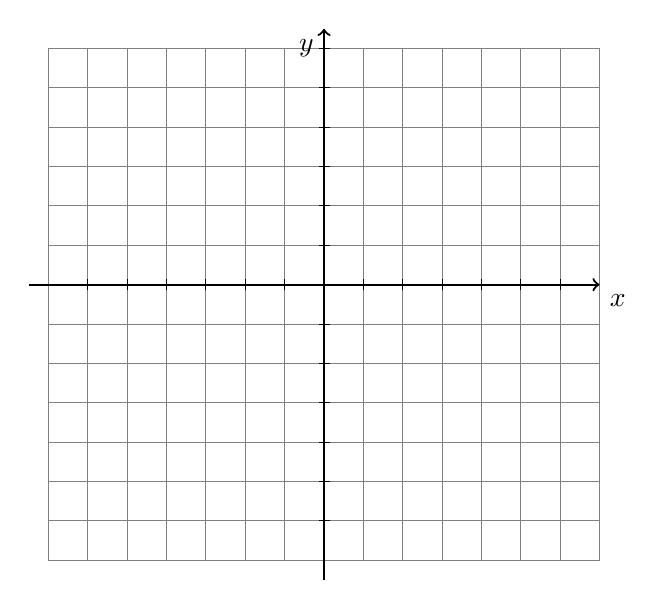
\begin{tikzpicture}[y=.5cm, x=0.5cm,font=\sffamily]
    %% ticks
    \draw[step = 1, gray] (-7,-7) grid (7,6);
    %% axis
    \draw[thick,->] (-7.5,0) -- coordinate (x axis mid) (7,0) node[anchor = north west] {$x$};
    \draw[thick,->] (0,-7.5) -- coordinate (y axis mid) (0,6.5) node[anchor = north east] {$y$};
    \foreach \y in {-6,-5,...,-1,1,2,...,6} {
      \draw (2pt, \y) -- (-2pt, \y);
    }
    \foreach \x in {-6,-5,...,-1,1,2,...,6} {
      \draw (\x,2pt) -- (\x,-2pt);
    }

\end{tikzpicture}



\item Determine an equation for the axis of symmetry.
\end{enumerate}



\vfill
\newpage

\item  Complete the square and use that work to find the vertex of the graph of the quadratic function.
$$y=5x^2-30x+49$$

%\item  You have a 500 foot roll of fencing and a large field.  You want to construct a rectangular playground area.  What are the dimensions of the largest such playground?  What is the largest area?
%\begin{enumerate}
%\item Draw a picture of the rectangular playground and label the side lengths using your own variables.
%\vfill
%\vfill
%\item Using your variables, write an equation that represents the area of the playground.
%\vfill
%\item Your previous answer should have two variables.  Use 500 to represent the perimeter of the the playground and solve for one of your variables.  (Note: all four sides of the rectangle will be used.)
%\vfill
%\vfill
%\item Rewrite your area equation in terms of only one variable and simplify.  The result should be a quadratic function.
%\vfill
%
%
%\newpage
%
%
%
%\item To determine the maximum area possible for the playground, what part of the parabola do you need to locate?
%\vfill
%
%\item Find that part of the parabola (from your previous answer).
%\vfill
%\vfill
%\item What is the largest area the playground could be?
%\vfill
%
%\item  What are the dimensions of that playground?
%\vfill
%
%\end{enumerate}
%
%
%




\end{enumerate}


